\documentclass[11pt, fleqn]{article}

\usepackage{amsmath}
\usepackage{amssymb}
\usepackage{amsthm}
\usepackage{mathtools}
\usepackage{hyperref}
\usepackage{ulem}
\usepackage{enumitem}
\usepackage[left=0.75in, right=0.75in, bottom=0.75in, top=1.0in]{geometry}
\usepackage{floatrow}
\usepackage{graphicx}
\usepackage[export]{adjustbox}

\usepackage{sectsty}
\sectionfont{\centering}

\usepackage[perpage]{footmisc}

\usepackage{fancyhdr}
\pagestyle{fancy}
\fancyhf{}
\lhead{190100036 \& 190100044 \& 190100055}
\rhead{CS 252: Lab 1}
\renewcommand{\footrulewidth}{1.0pt}
\cfoot{Page \thepage}

\setlength{\parindent}{0em}
\renewcommand{\arraystretch}{2}%

\title{CS 252: Lab 1}
\author{
\begin{tabular}{|c|c|c|}
     \hline
     Krushnakant Bhattad & Devansh Jain & Harshit Varma \\
     \hline
     190100036 & 190100044 & 190100055 \\
     \hline
\end{tabular}
}
% \author{
%   Krushnakant Bhattad\\
%   190100036
%   \and
%   Devansh Jain\\
%   190100044
%   \and
%   Harshit Varma\\
%   190100055
% }
\date{\today}

\usepackage{hyperref}

\usepackage[dvipsnames]{xcolor}

\begin{document}

\maketitle
\tableofcontents
\thispagestyle{empty}
\setcounter{page}{0}
\renewcommand{\arraystretch}{1}

\vspace{5em}
\section*{About the report}
Due to Covid-19 pandemic restrictions, only Devansh was able to take the measurements over a path of more than 1 km. This data was used to answer \nameref{parta}, \nameref{partb} and \nameref{partc}. \\
Harshit and Krushnakant did the measurements at (different) fixed locations independently. Harshit's data was used to answer \nameref{partd} and Krushnakant's data is present in the Appendix (Figure \ref{fig:part_d_extra}). \\
All the team members contributed to the analysis and discussions for all the parts.\\
Android App Net Monitor Lite was used for collecting the data and Android App Opensignal was used to get the location and information about the cell towers located nearby. For plotting and a basic analysis of the data, \texttt{Python-3} was used.

\newpage 
\section*{Part (a)}
\label{parta}
\addcontentsline{toc}{section}{Part (a)}
\setcounter{equation}{0}

\textit{Record signal strength over some geographical area,
and pictorially represent it on a map. Use colours to say if the signal strength is good or bad etc. State the range of signal strengths (in dBm) which correspond to different colours. (15 marks)}

\begin{figure}[H]
    \centering
    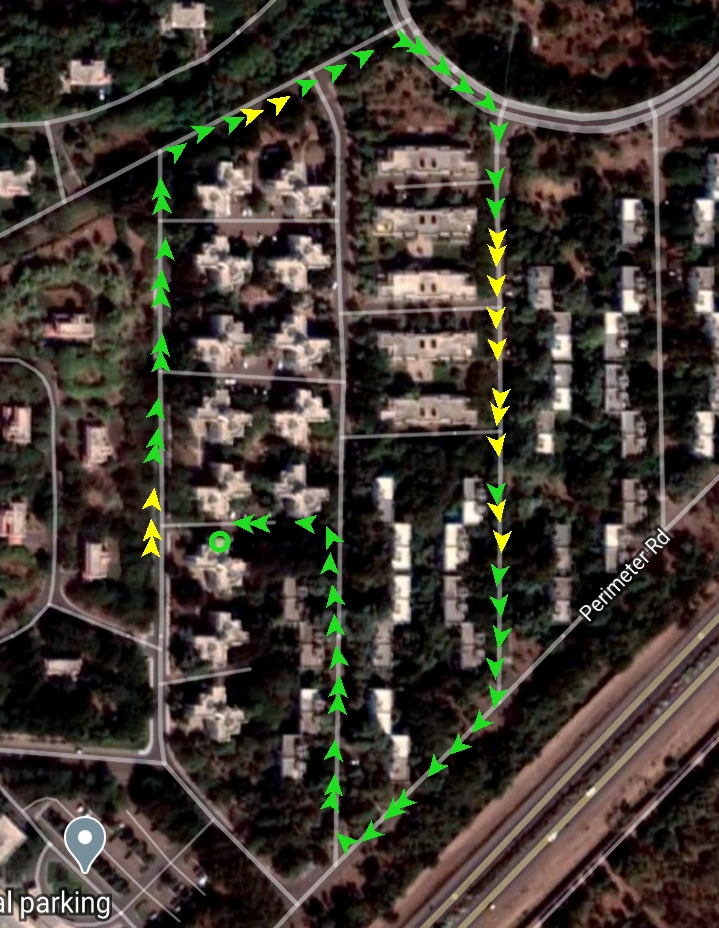
\includegraphics[scale = 0.6]{path_map.jpg}
    \caption{Area over which the signal strength was recorded}
    \label{fig:path_map}
\end{figure}

\subsection*{Color Scheme:} 
In the above map, the parts of the path covered by \textcolor{ForestGreen}{green} arrows
indicate a good signal strength; 
while those covered by \textcolor{Apricot}{yellow} indicate 
a relatively bad signal strength.\\

The signals received varied from \textbf{-92} dBm\footnote{dBm:  decibels per milliwatt} to \textbf{-52} dBm, with a mean of \textbf{-74.11} dBm and a standard deviation of \textbf{9.66} dBm

\subsection*{Ranges covered by different colours:}

\textcolor{ForestGreen}{green} covers the range \textbf{-50 dBm} to \textbf{-85 dBm}\\
\textcolor{Apricot}{yellow} covers the range \textbf{-85 dBm} to \textbf{-105 dBm}

\vspace*{\fill}
\begin{figure}[H]
    \centering
    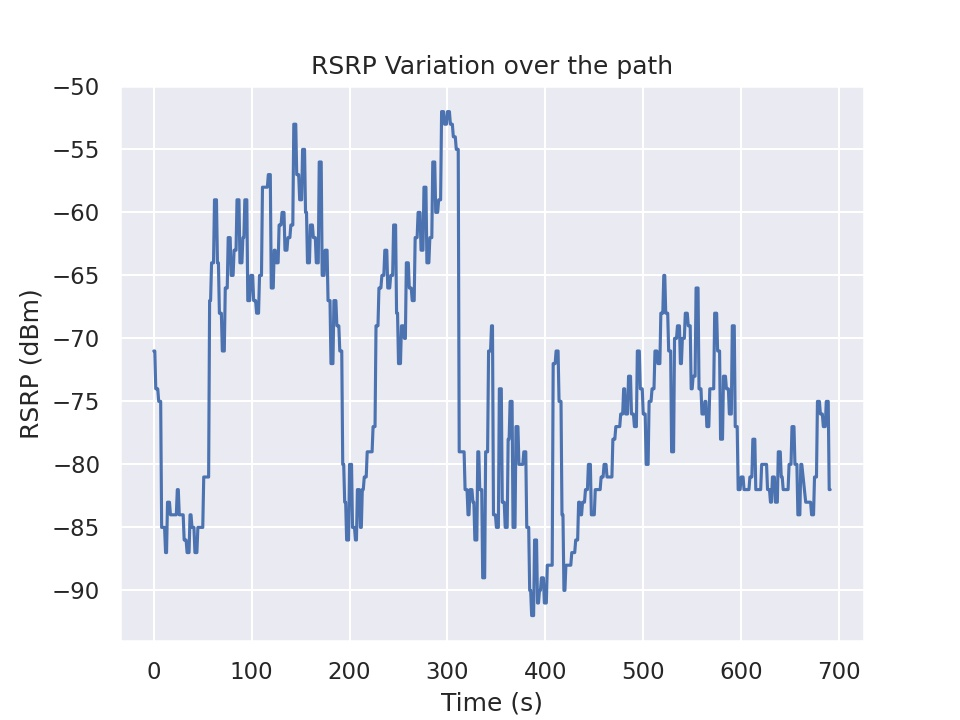
\includegraphics[scale = 1]{part_a.jpg}
    \caption{RSRP Variation over the path}
    \label{fig:part_a}
\end{figure}
\vspace*{\fill}

\newpage
\section*{Part (b)}
\label{partb}
\addcontentsline{toc}{section}{Part (b)}
\setcounter{equation}{0}

\textit{Make a list of all the unique base-stations (\texttt{eNodeBIDs}) your phone was connected to, during the measurement. (5 marks)}

\medskip

The set of eNBIDs that the phone connected to are: 
$\mathbf{\{ 5318, 5482, 6378, 12987, 13532 \}}$\\

\begin{figure}[H]
    \centering
    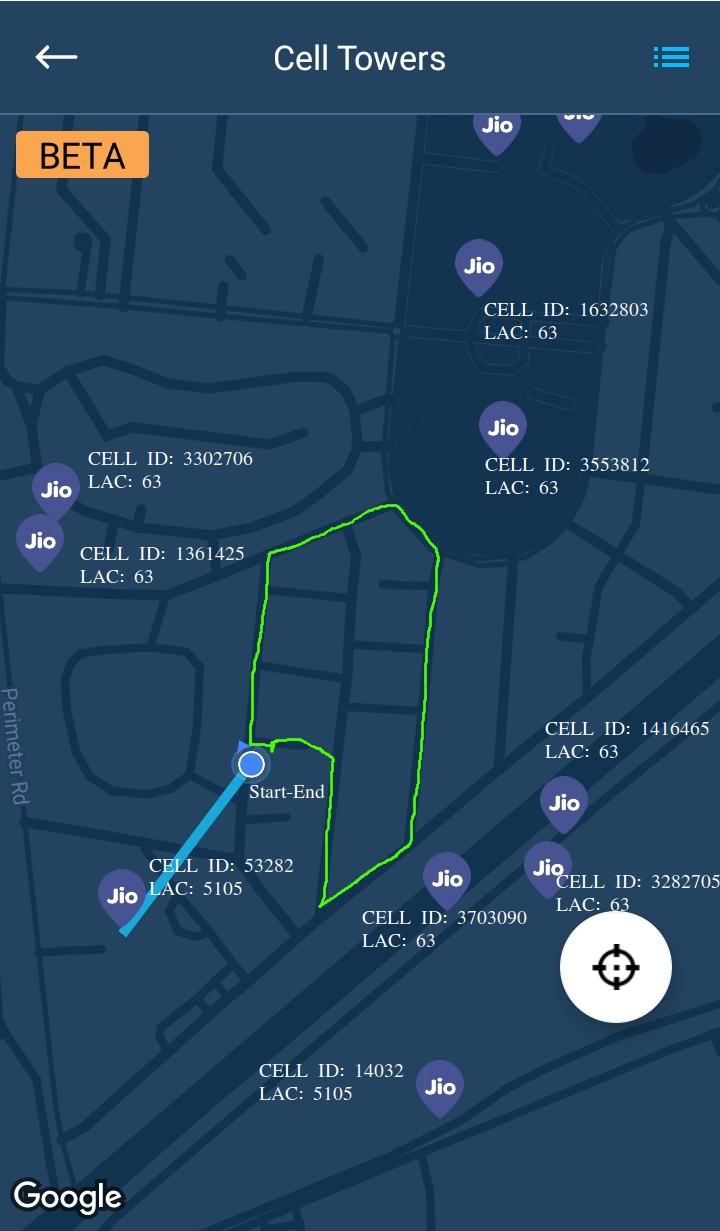
\includegraphics[scale = 0.4]{part_b.jpg}
    \caption{Annotated Cell Towers}
    \label{fig:part_b}
\end{figure}


\newpage
\section*{Part (c)}
\label{partc}
\addcontentsline{toc}{section}{Part (c)}
\setcounter{equation}{0}

\textit{State in words in your report what you think the reasons for poor signal strength were. If you can annotate your map to show obstacles etc, that would be even better, but this is not essential. (5 marks)}\\

The yellow signal patch present on the downward journey in Figure \ref{fig:path_map} can be explained as a consequence of the following two reasons:
\begin{enumerate}
    \item The path on both sides has \textbf{tall buildings} and it is a street road and when we crosscheck it with locations of Base Stations in Figure \ref{fig:part_b}, we can see that they offer obstruction.
        
    \begin{figure}[H]
        \centering
        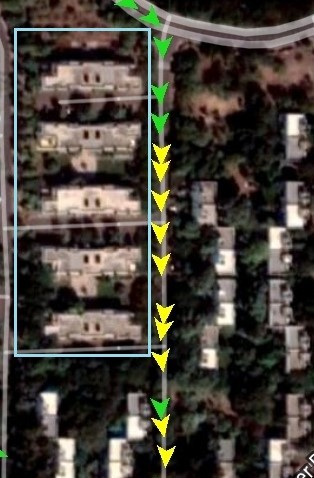
\includegraphics[scale = 0.5]{zoomed_path.jpg}
        \caption{Tall buildings obstruct the signals}
    \end{figure}
    
    \item Another possible reason which can be seen by analyzing Figure \ref{fig:part_b} is that there are no close by base stations (as compared to the previous path segments) and three to four base stations are almost equally spaced from the path
    
    \begin{figure}[H]
        \centering
        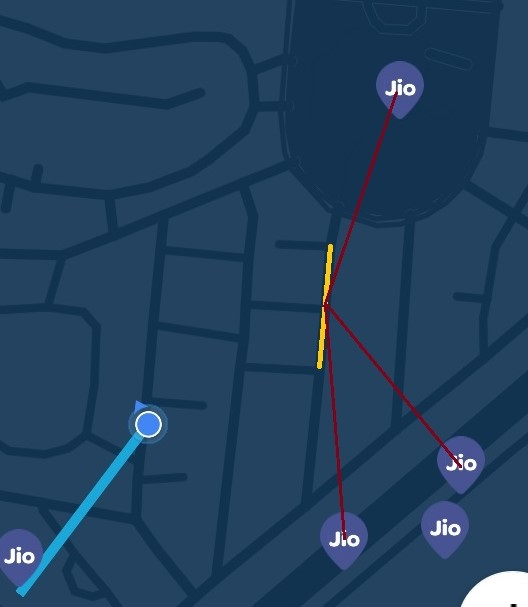
\includegraphics[scale = 0.5]{far_away.jpg}
        \caption{Closest base stations when signal is low}
    \end{figure}
    
\end{enumerate}
The first reason seems to be more influential as there is a significant dip in signal compared to other regions.



\newpage
\section*{Part (d)}
\label{partd}
\addcontentsline{toc}{section}{Part (d)}
\setcounter{equation}{0}

\textit{Comment if when you are standing in a fixed location (when you are not moving) if the signal strength (RSRP: reference signal received power) is steady or if it varies, based on a measurement of a minute’s duration. Give a plot of how RSRP varies with time at a fixed location. (5 marks)}

\begin{figure}[H]
    \centering
    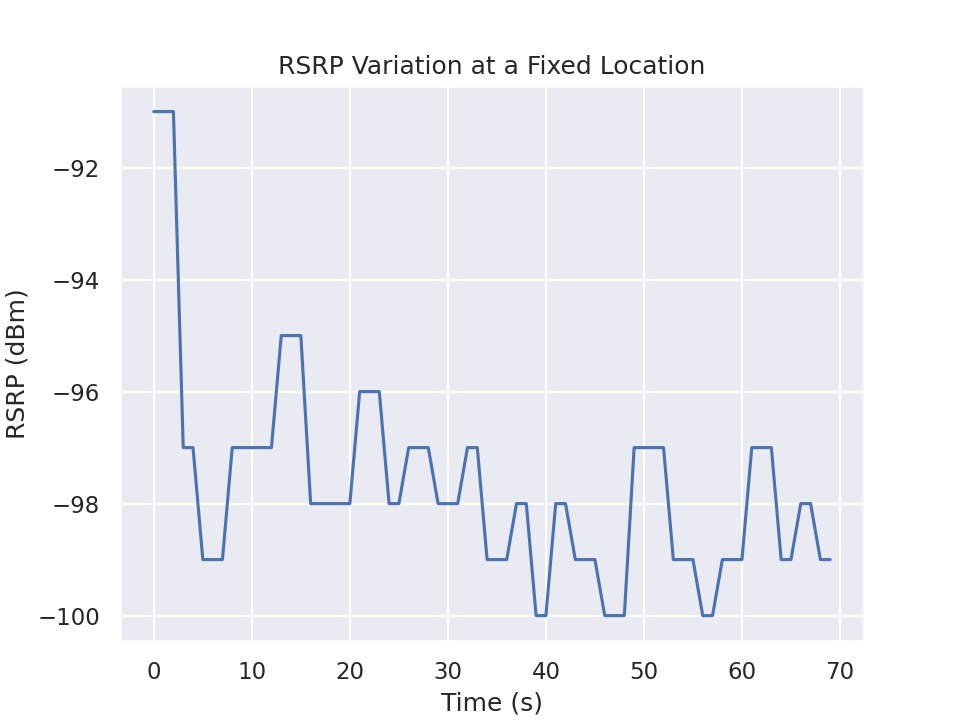
\includegraphics[scale = 1]{part_d.jpg}
    \caption{RSRP Variation at a Fixed Location}
\end{figure}

While standing at a fixed location 
\footnote{Measurements were taken in a confined space} 
for about 70 seconds, the signal strength varies between \textbf{-100} and
\textbf{-91} dBm, having a mean value of \textbf{-97.69} dBm and a standard deviation of \textbf{1.89} dBm\\

Another set of findings (obtained while standing at a \textbf{different} fixed location for about 70 seconds), with a mean of \textbf{-84.25} dBm and a standard deviation of \textbf{1.34} dBm is plotted in Figure \ref{fig:part_d_extra}. \\

This is still much less than the variation seen in \nameref{parta}, which varied from -92 dBm to -52 dBm, with a mean of -74.11 dBm and a standard deviation of 9.66 dBm\\

We believe that this small variation, seen at a fixed location can be attributed to:
\begin{enumerate}[itemsep=-1ex]
    \item Local interference from neighbouring devices
    \item Natural noise while data acquisition 
\end{enumerate}


\newpage
\section*{Appendix}
\addcontentsline{toc}{section}{Appendix}
\setcounter{equation}{0}

\subsection*{Screenshots}
\begin{figure}[H]
    \centering
    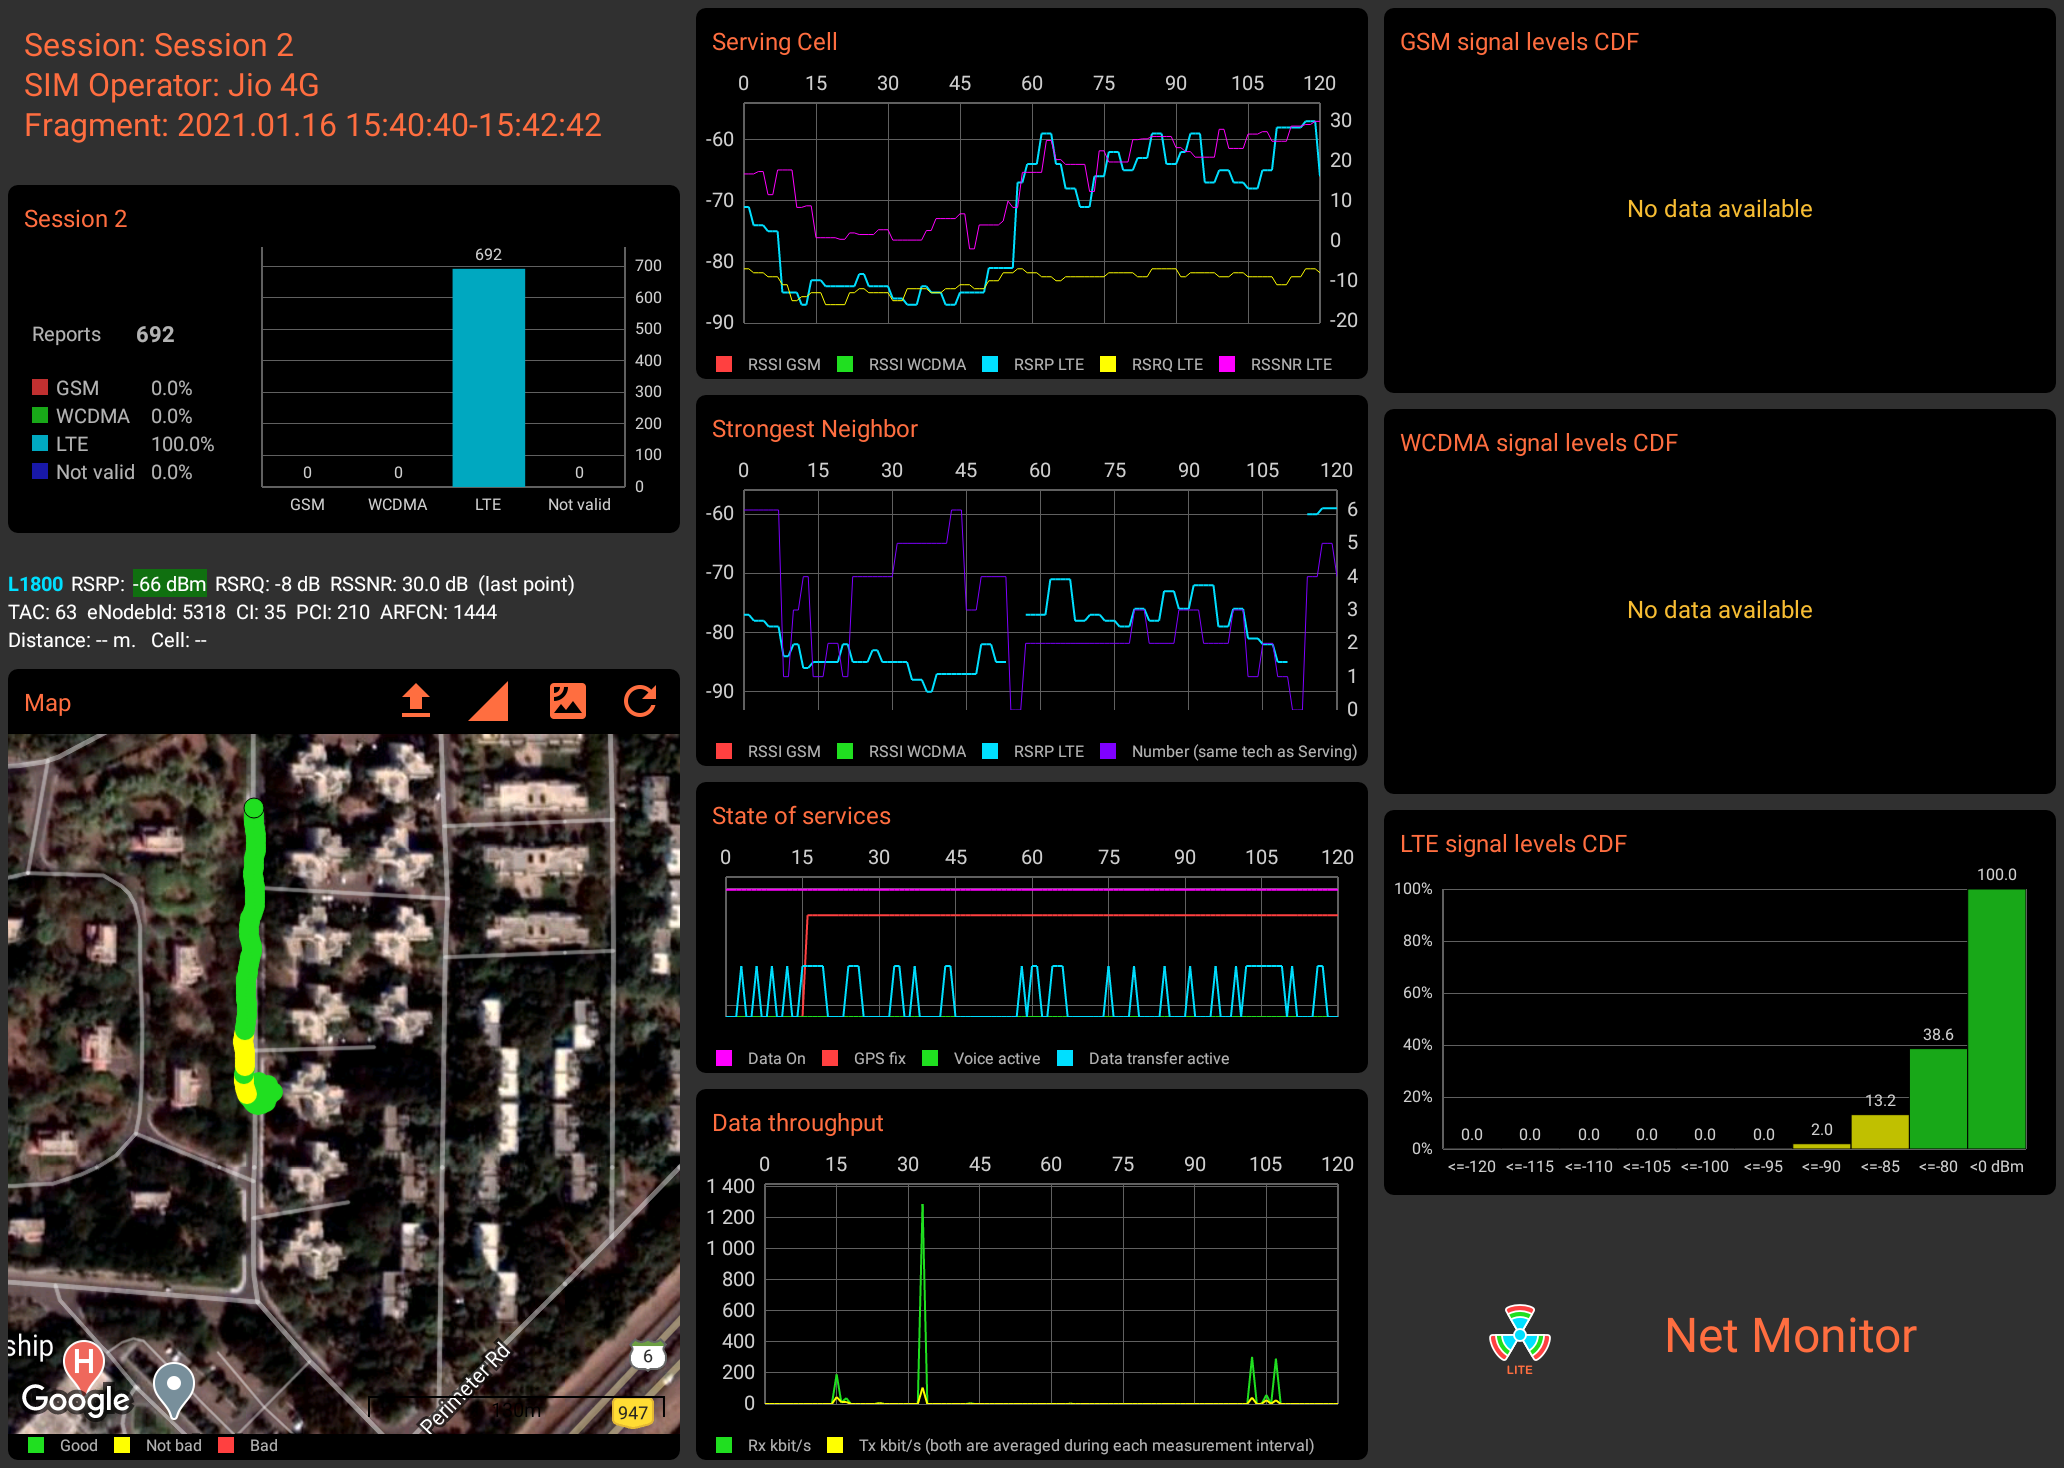
\includegraphics[scale = 0.18]{part_a_screenshot_1.png}
    \caption{Net Monitor Data over Path (1)}
\end{figure}
\begin{figure}[H]
    \centering
    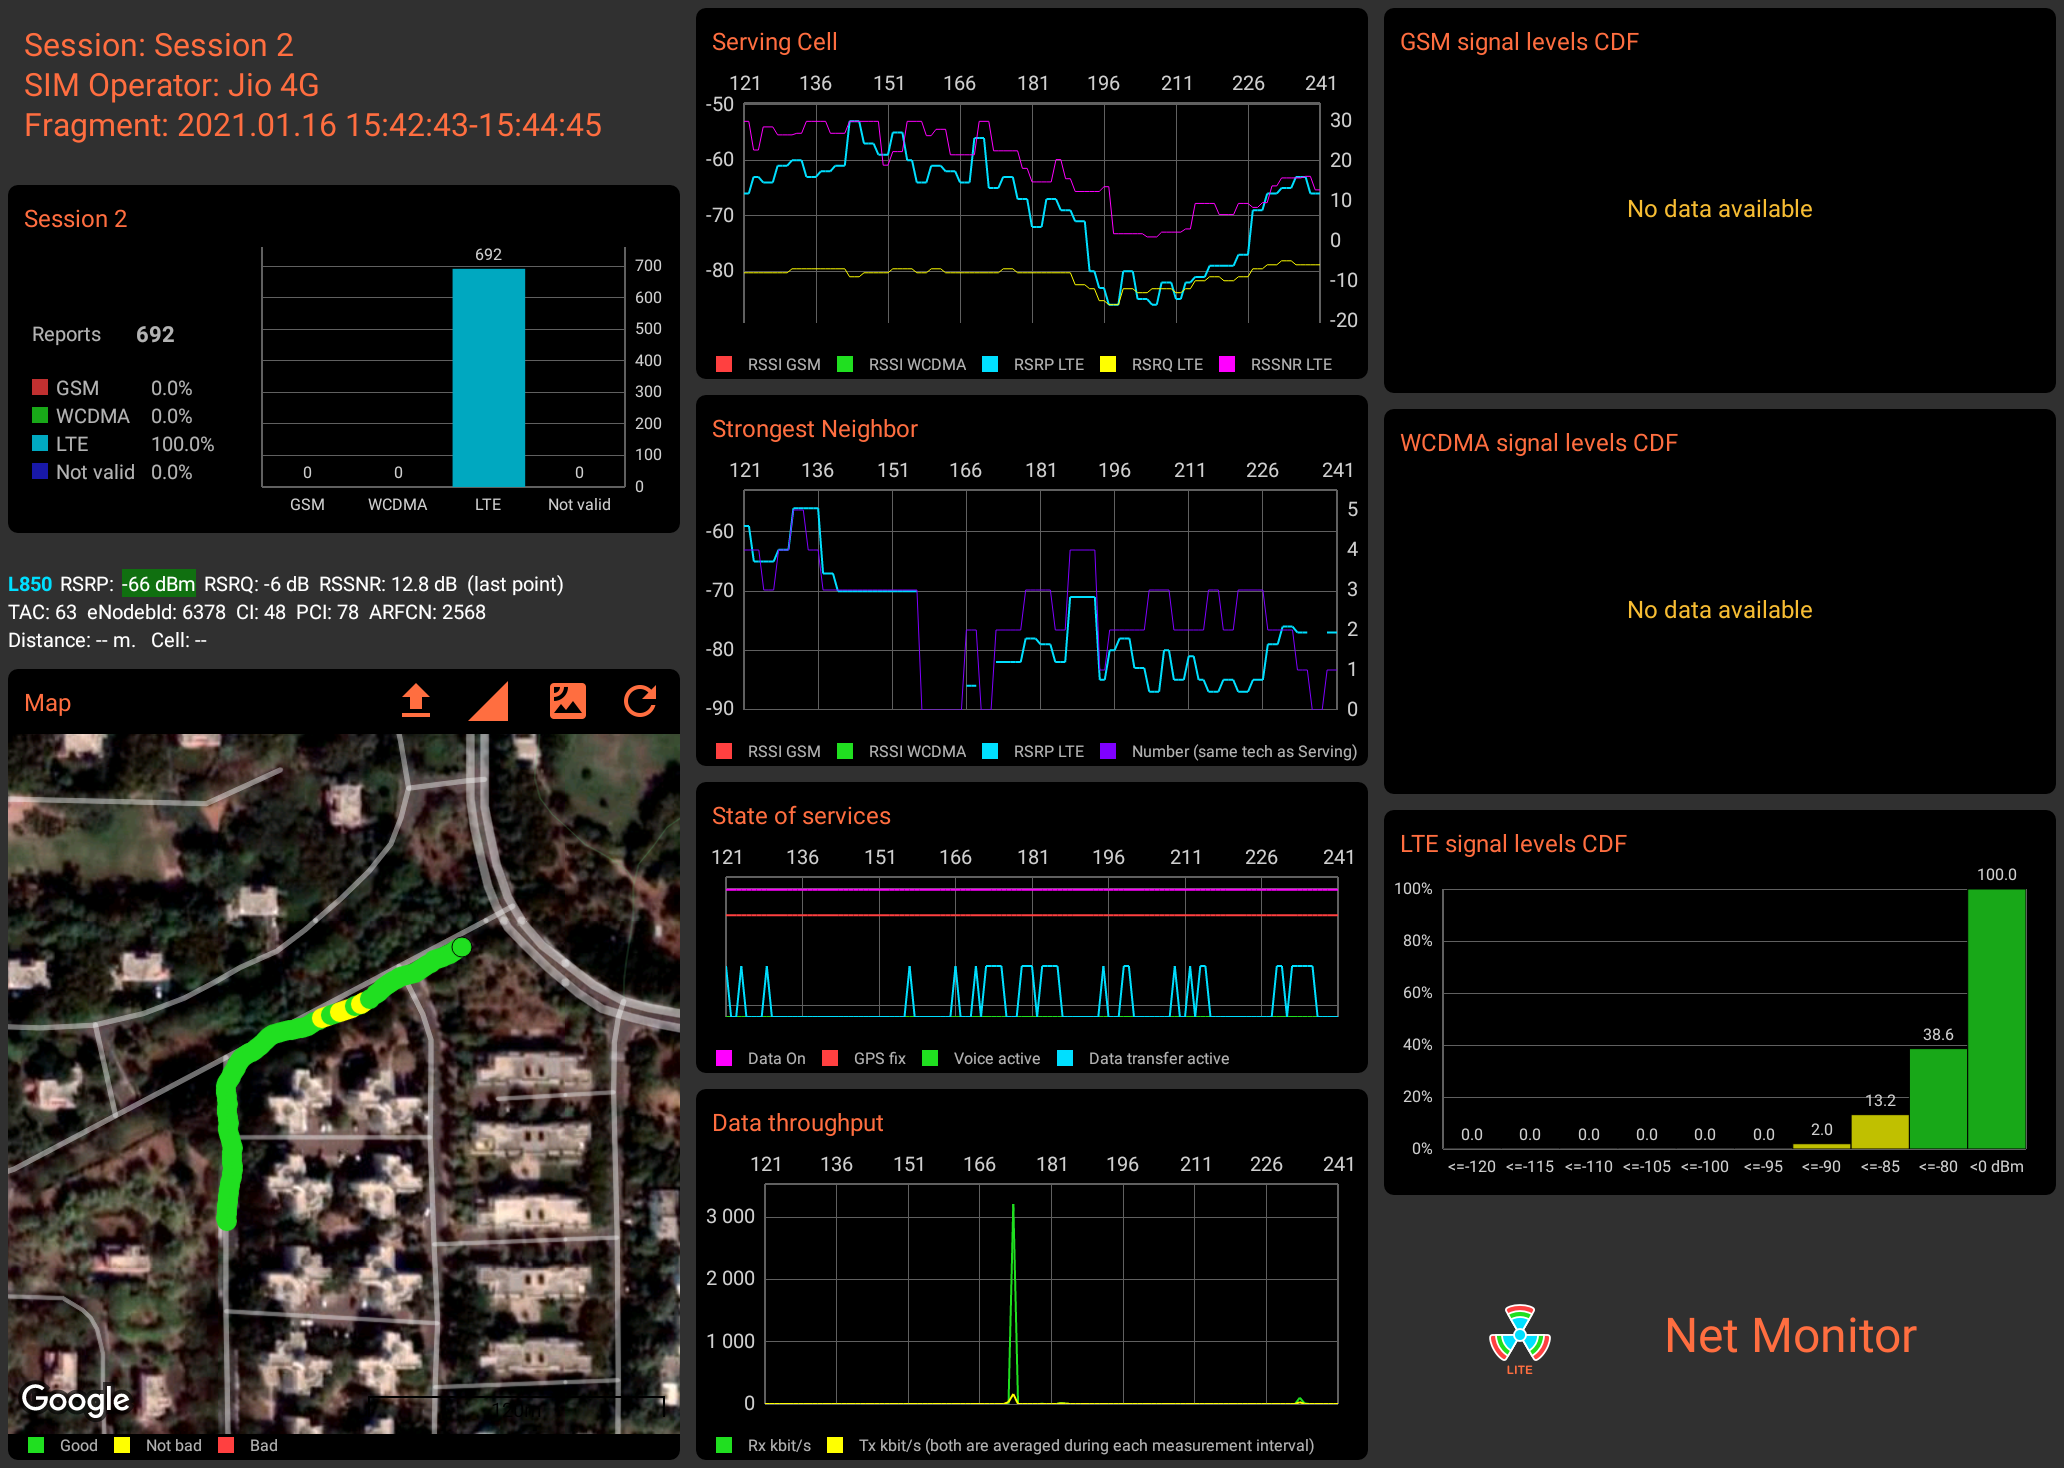
\includegraphics[scale = 0.18]{part_a_screenshot_2.png}
    \caption{Net Monitor Data over Path (2)}
\end{figure}
\begin{figure}[H]
    \centering
    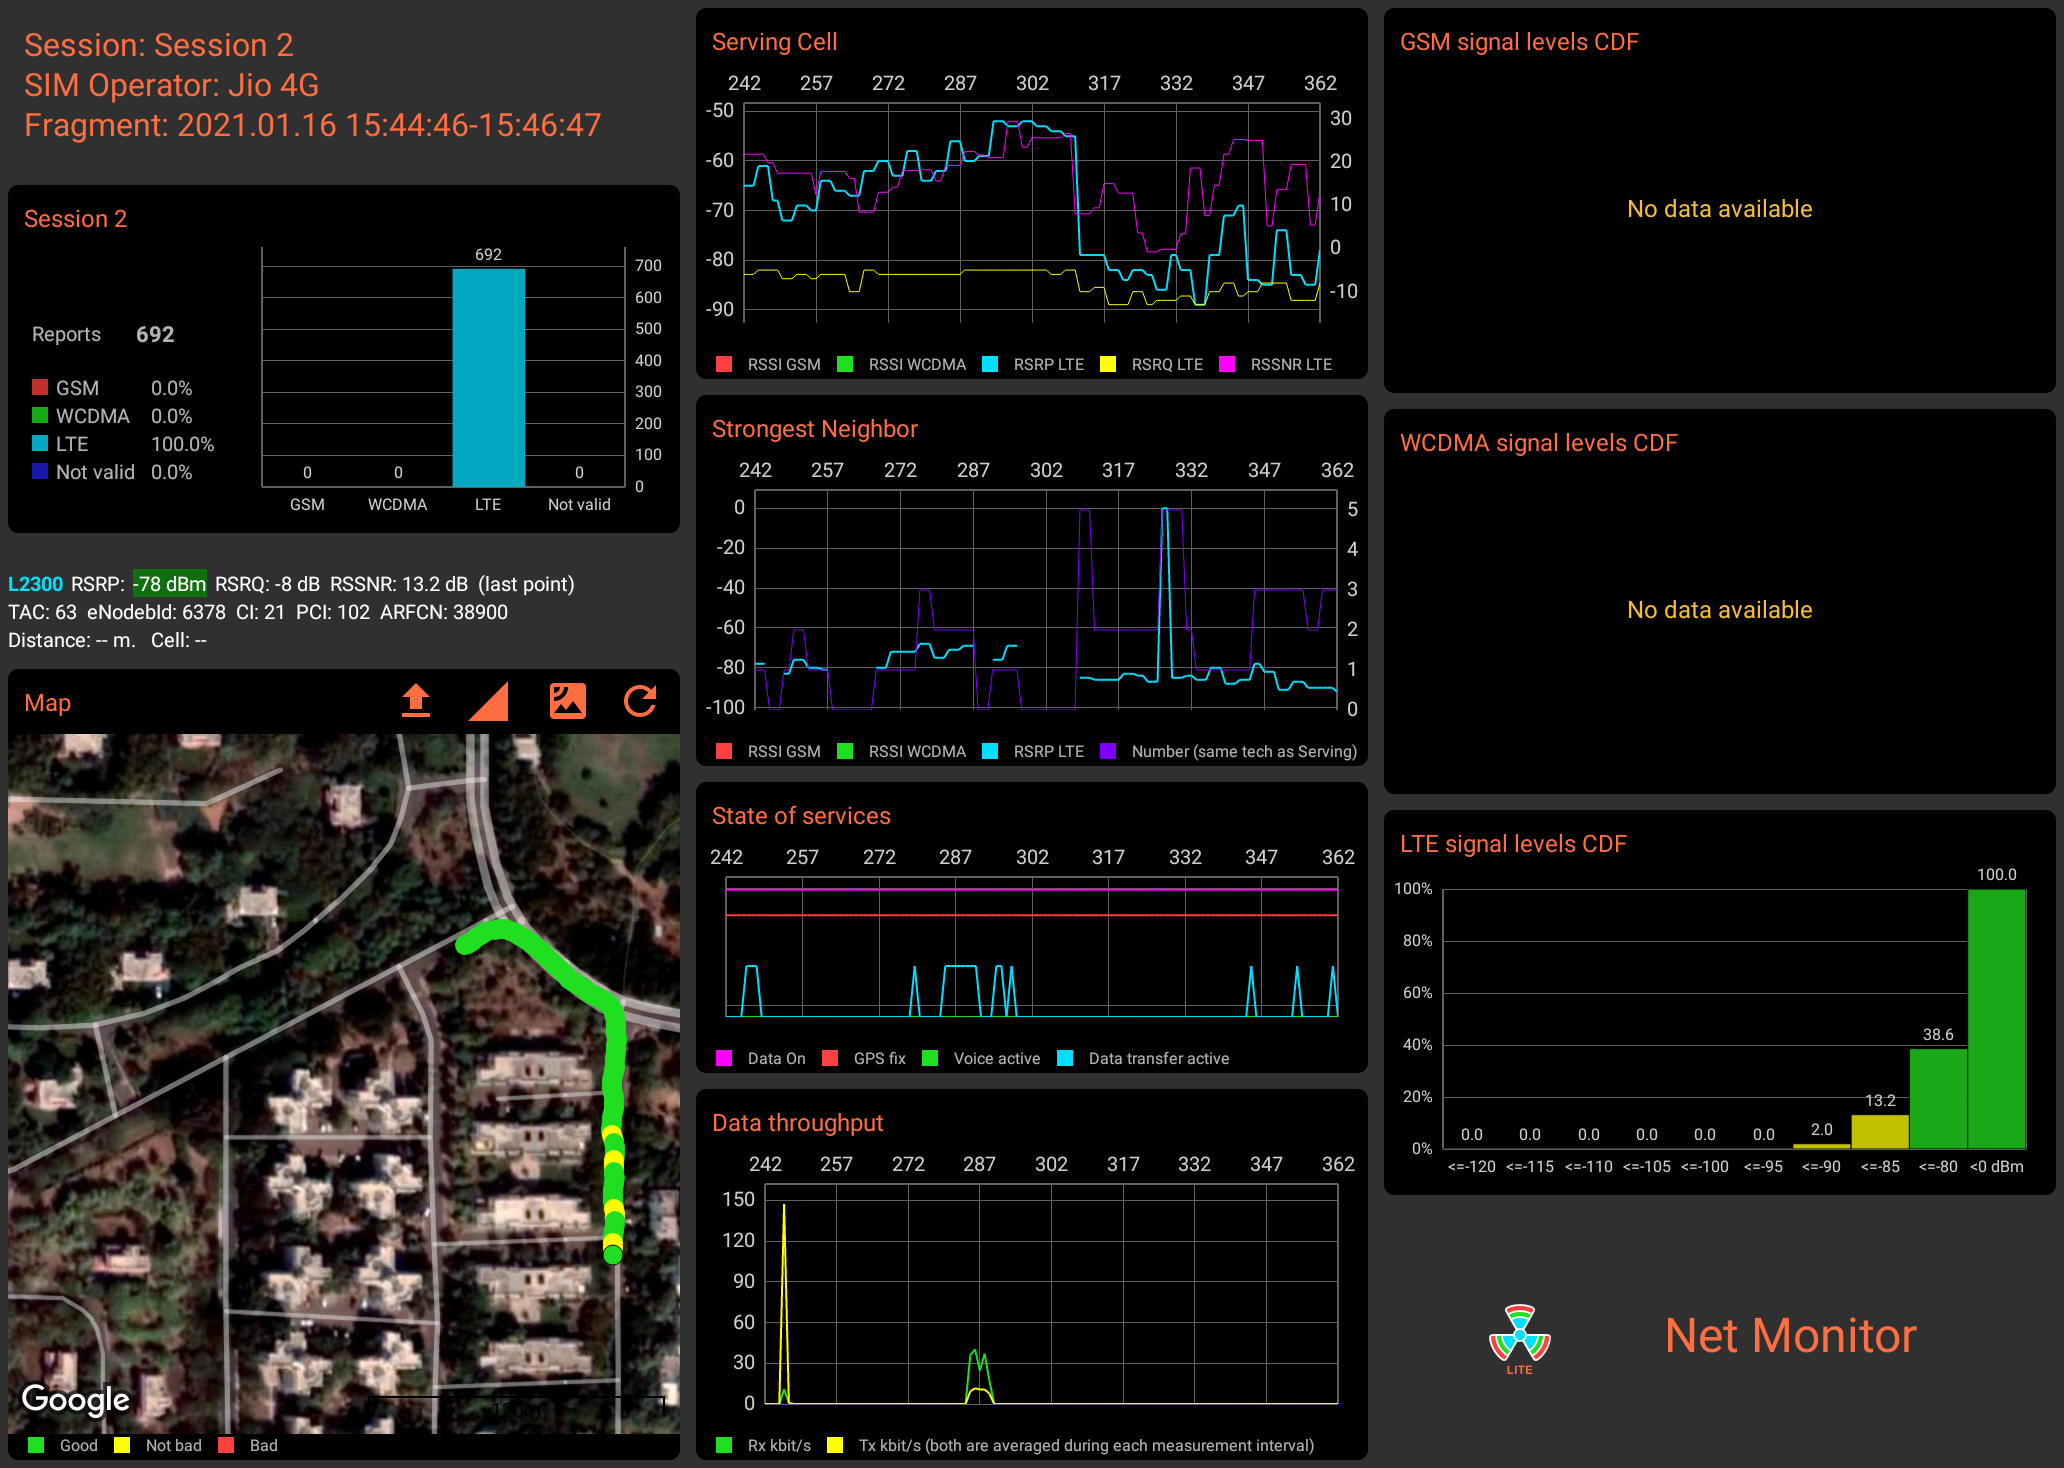
\includegraphics[scale = 0.18]{part_a_screenshot_3.png}
    \caption{Net Monitor Data over Path (3)}
\end{figure}
\begin{figure}[H]
    \centering
    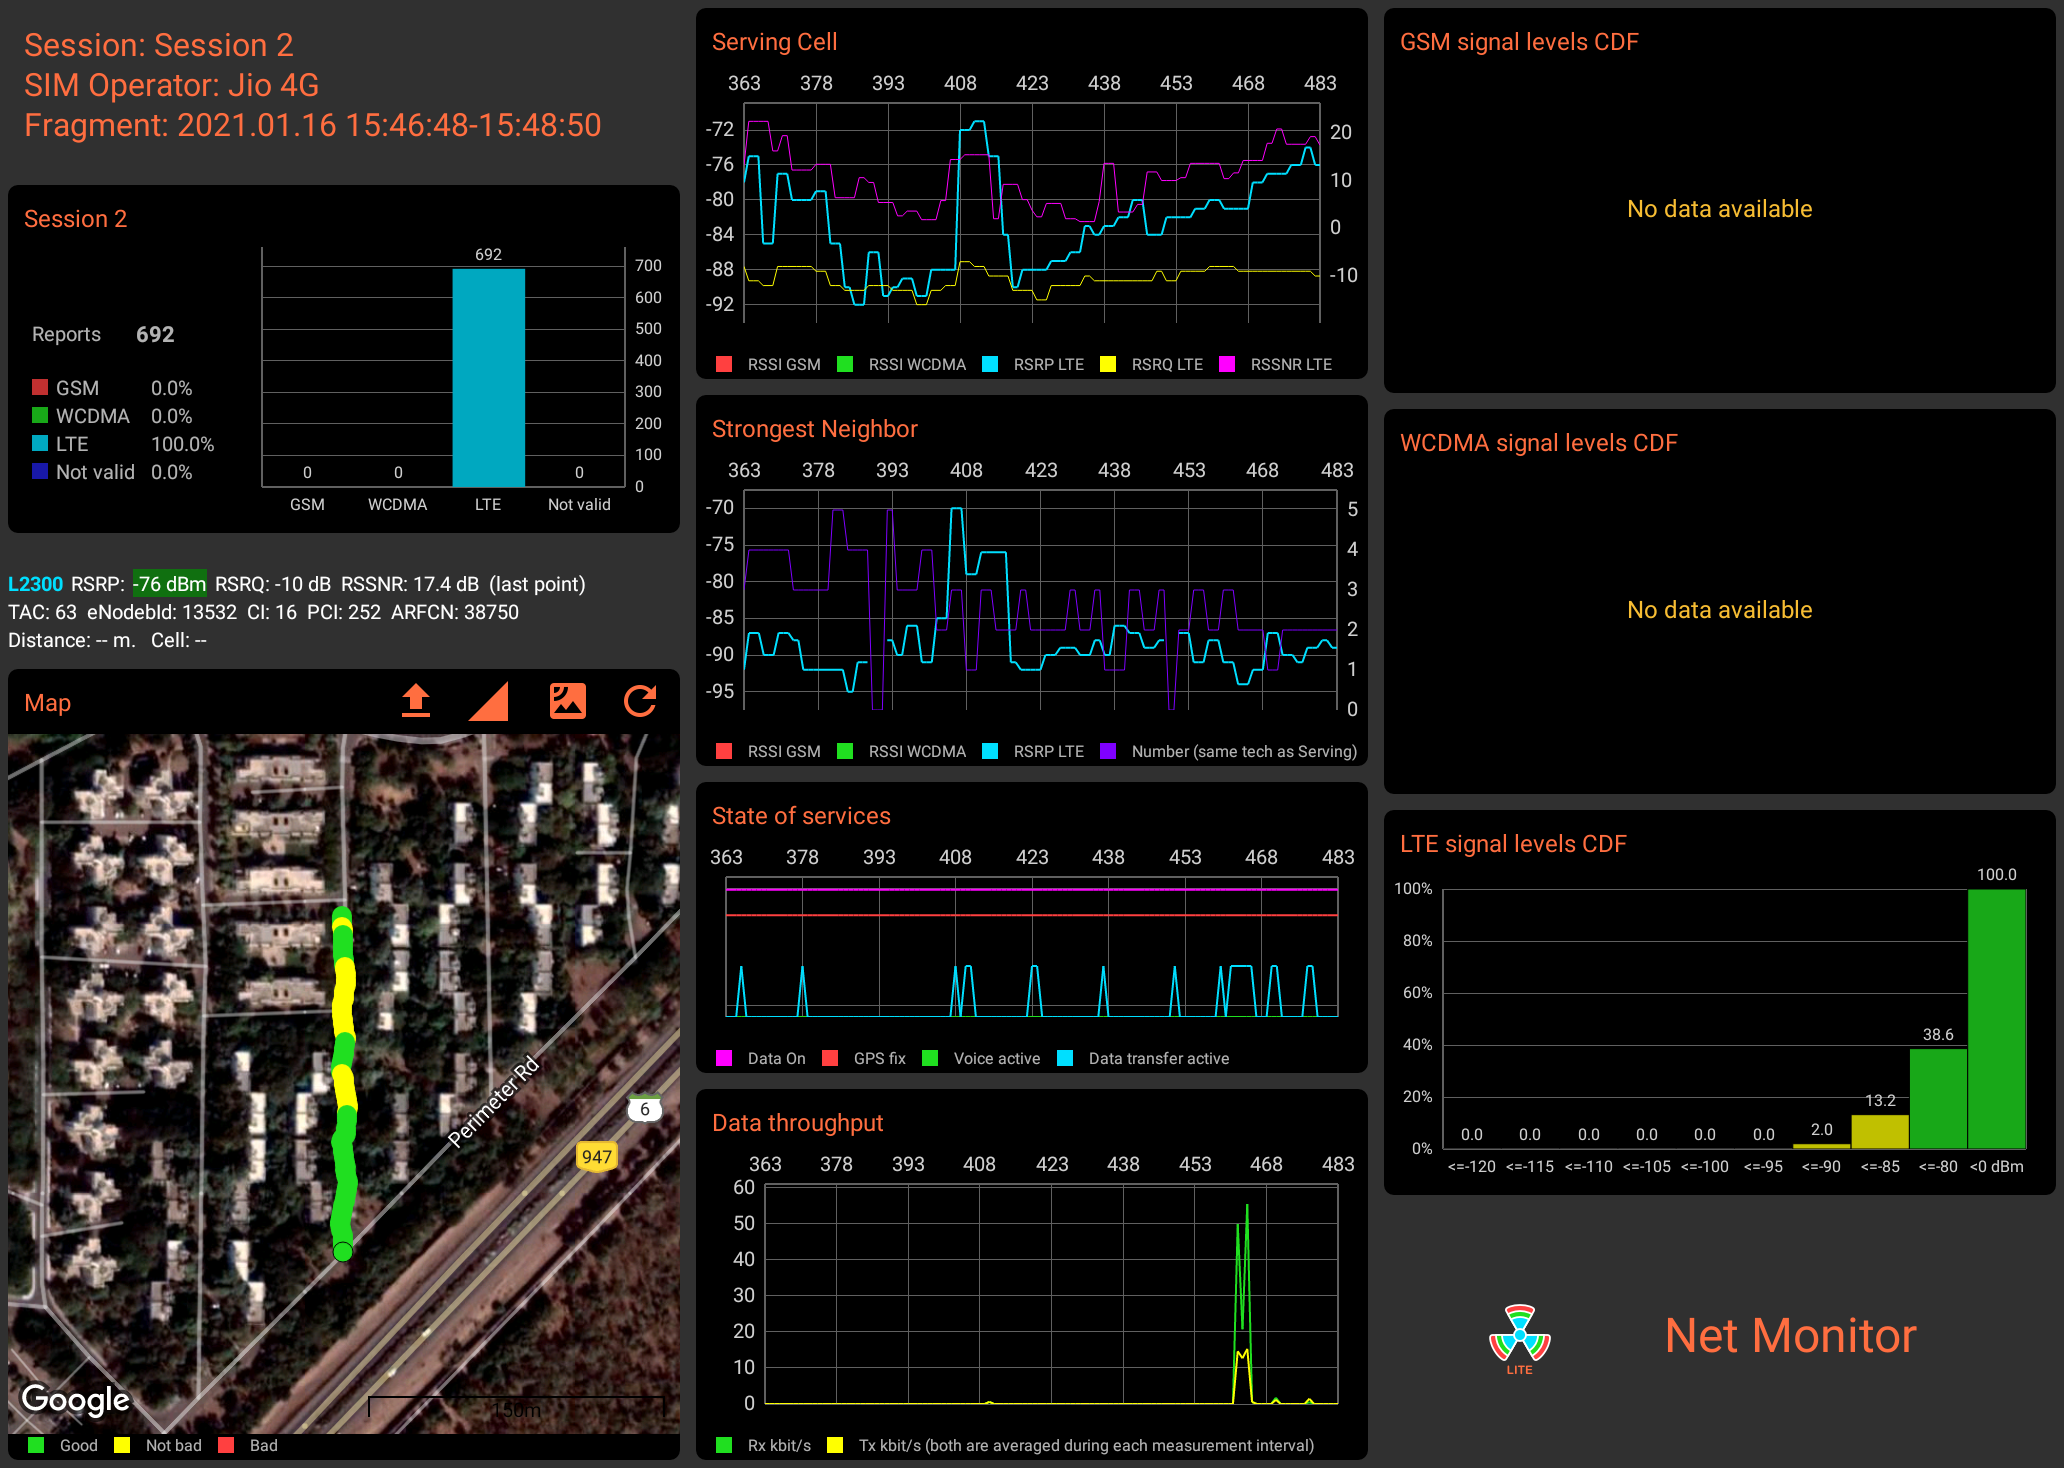
\includegraphics[scale = 0.18]{part_a_screenshot_4.png}
    \caption{Net Monitor Data over Path (4)}
\end{figure}
\begin{figure}[H]
    \centering
    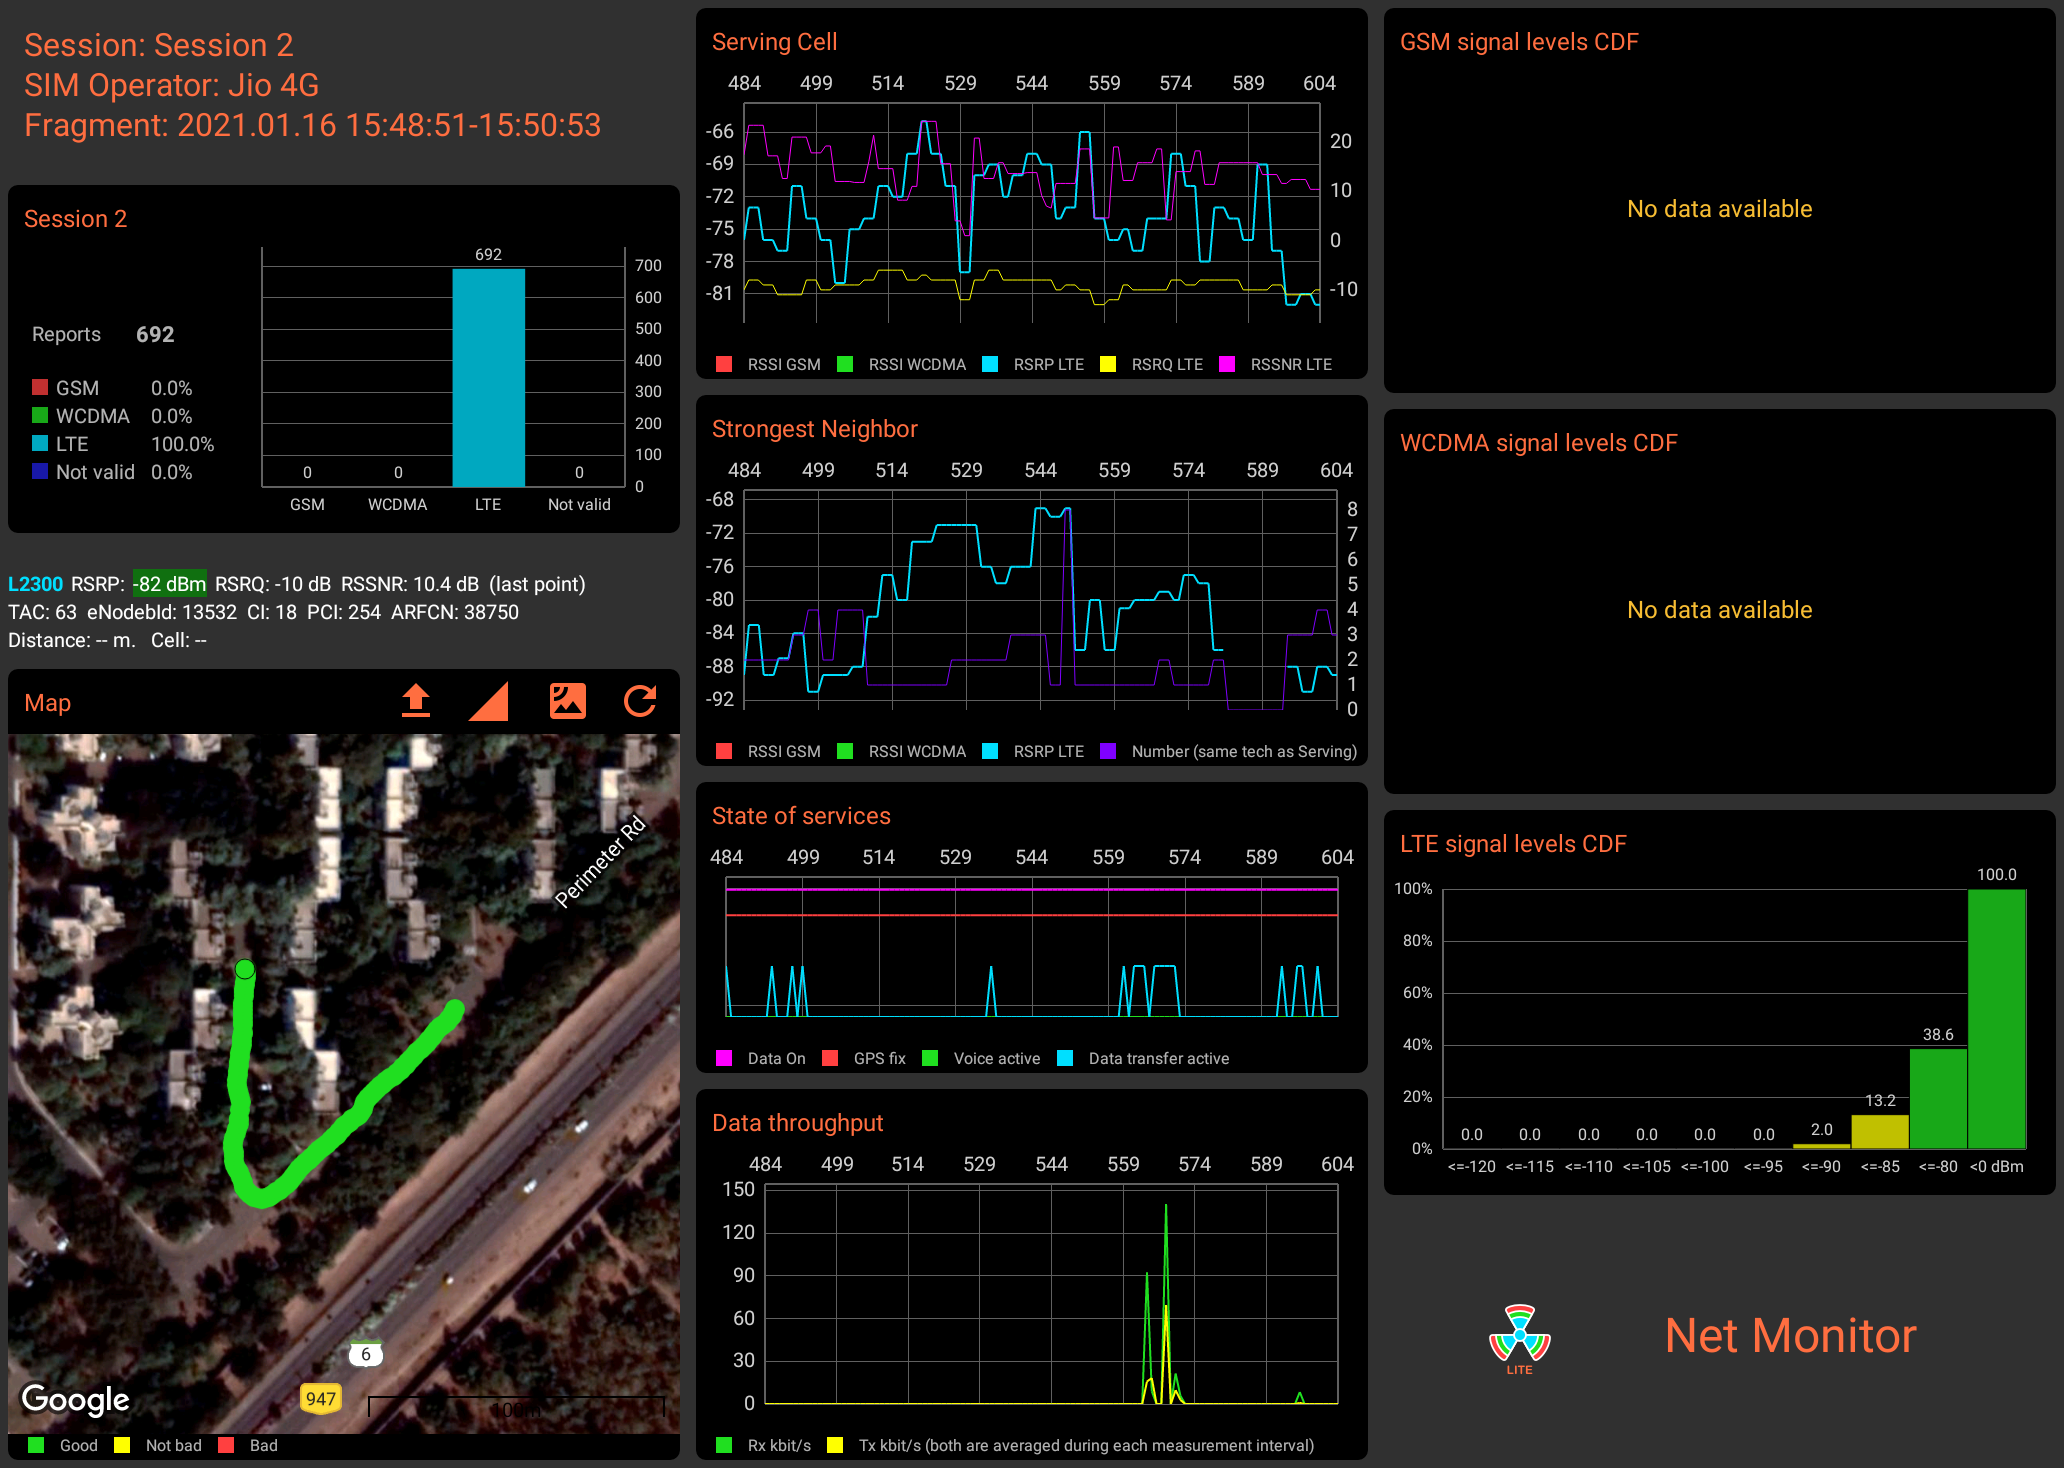
\includegraphics[scale = 0.18]{part_a_screenshot_5.png}
    \caption{Net Monitor Data over Path (5)}
\end{figure}
\begin{figure}[H]
    \centering
    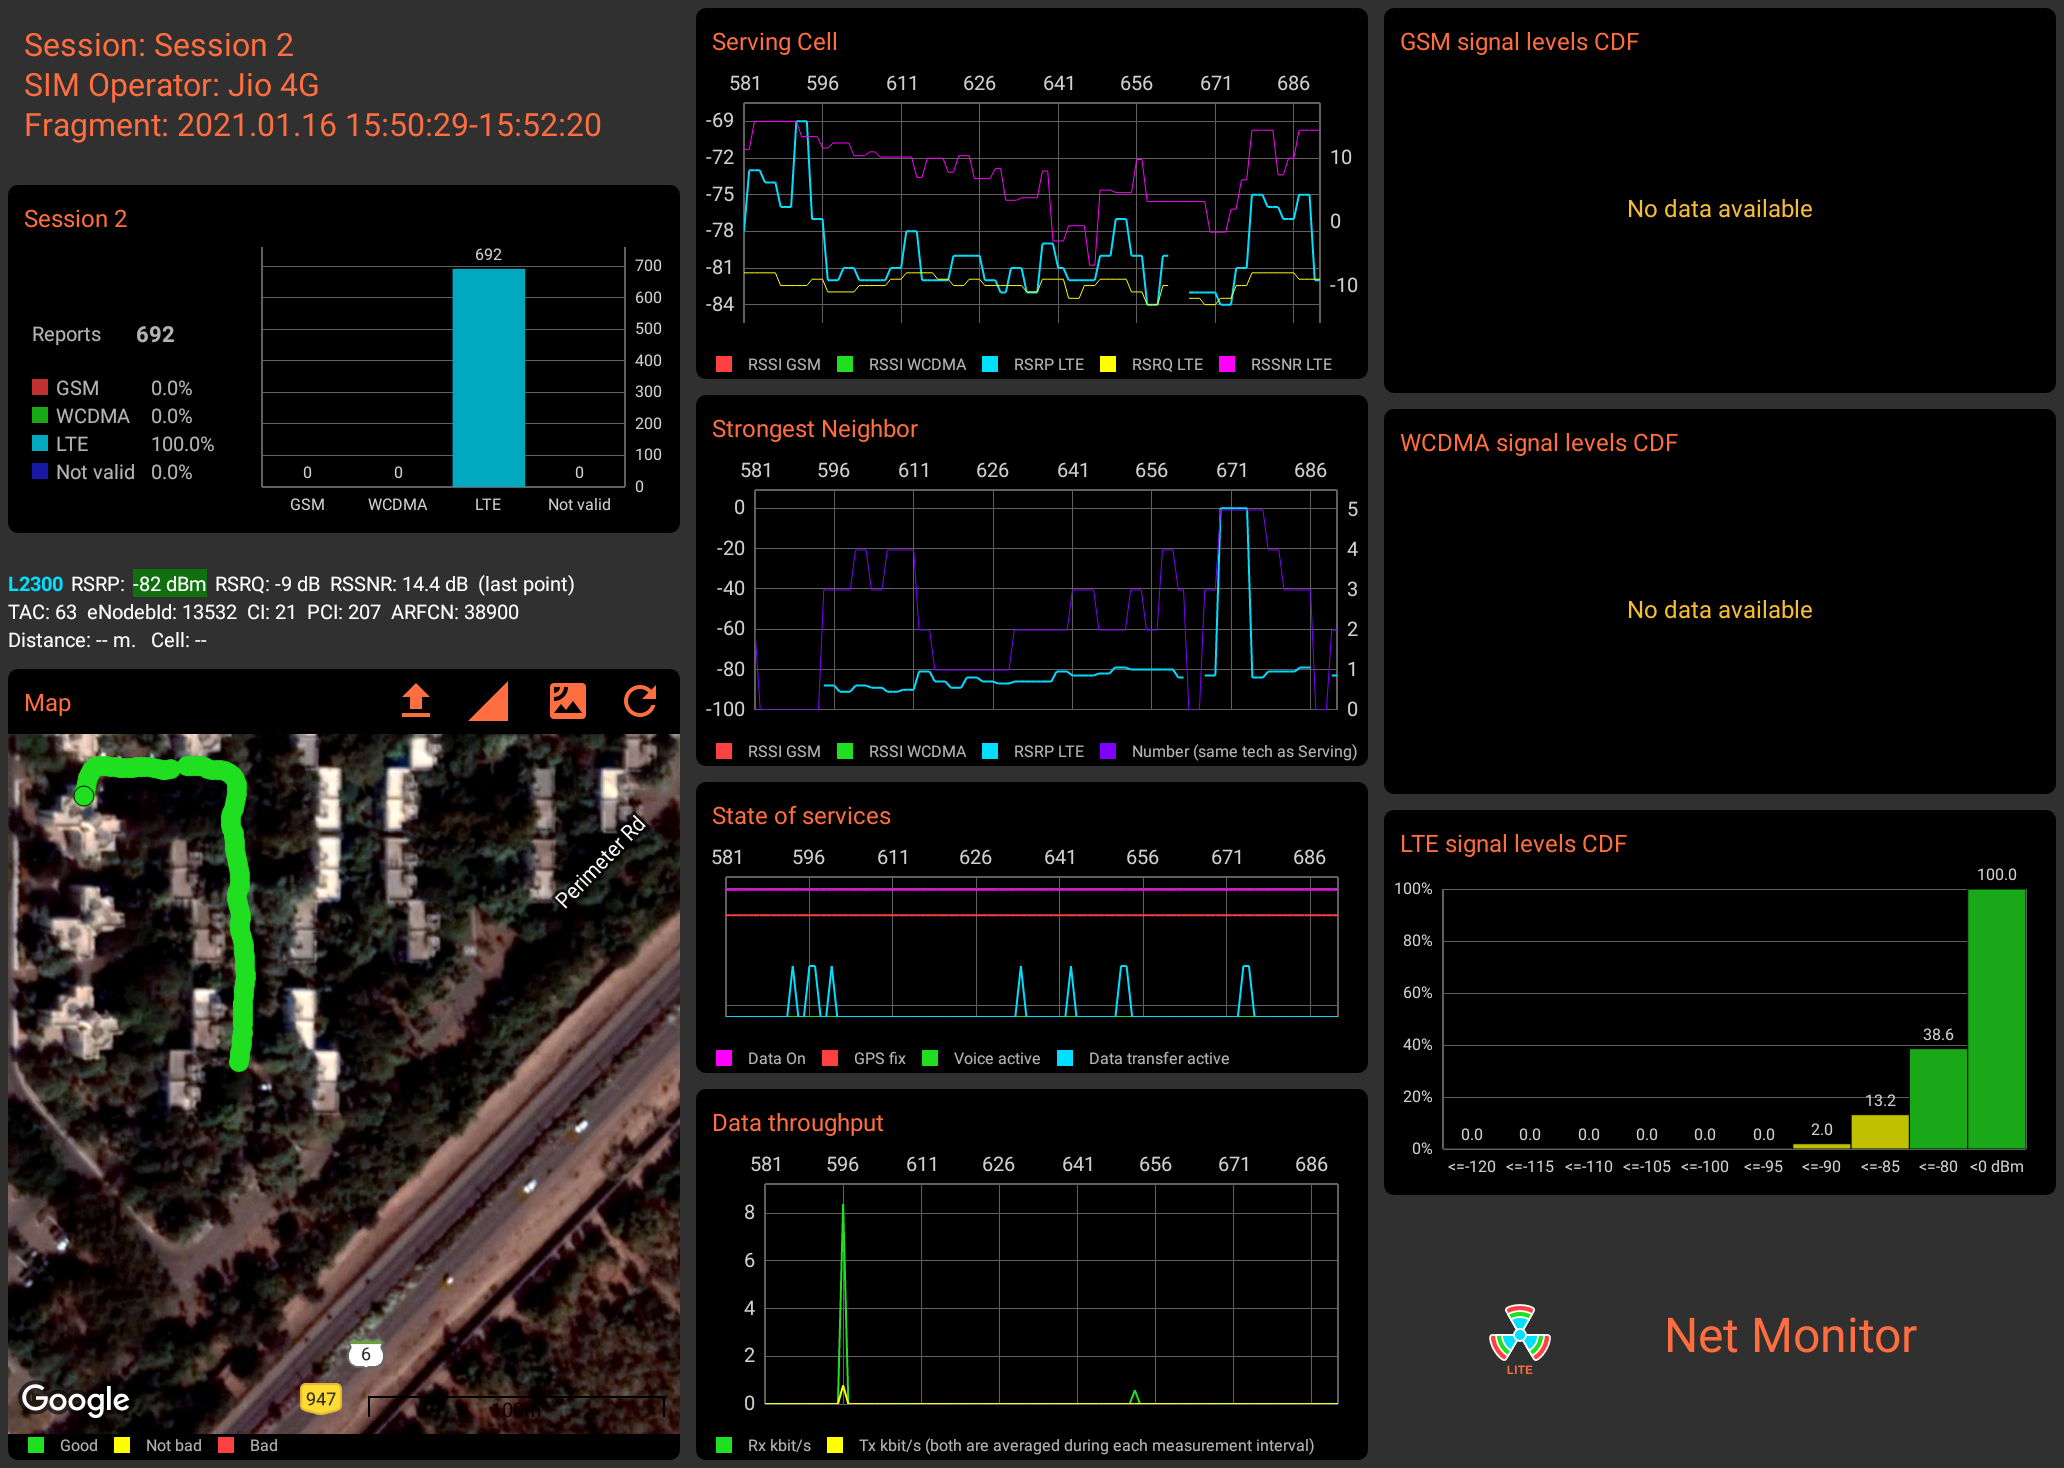
\includegraphics[scale = 0.18]{part_a_screenshot_6.png}
    \caption{Net Monitor Data over Path (6)}
\end{figure}
\begin{figure}[H]
    \centering
    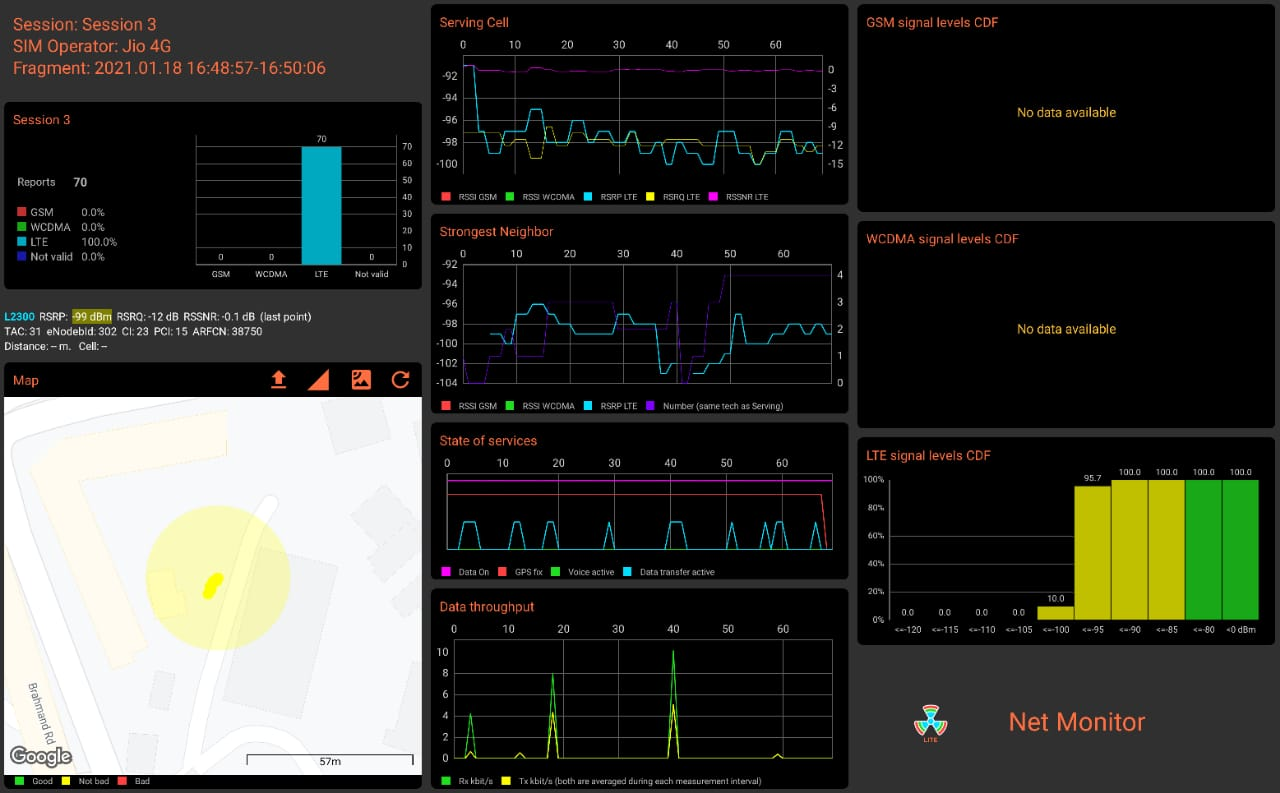
\includegraphics[scale = 0.36]{part_d_screenshot.jpg}
    \caption{Net Monitor Data at a Fixed Location}
\end{figure}

\begin{figure}[H]
    \centering
    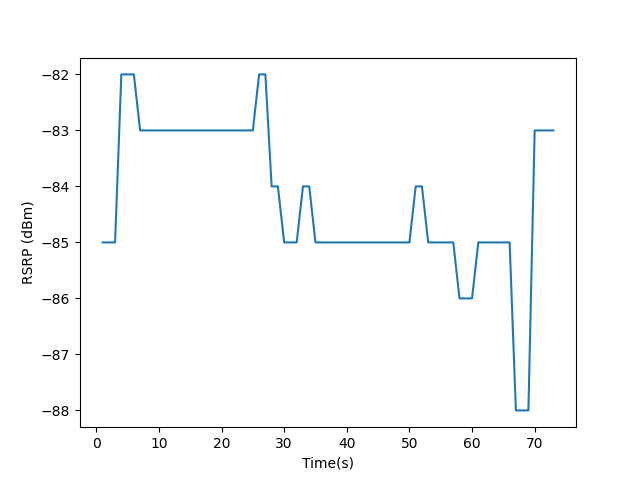
\includegraphics[scale = 0.7]{part_d_extra.png}
    \caption{RSRP Variation at a Fixed Location}
    \label{fig:part_d_extra}
\end{figure}

\end{document}